\documentclass[nobib]{tufte-handout}

\title{Lecture 3: Common graph families, trees, and Cayley's theorem $\cdot$ 1MA020}

\author[Vilhelm Agdur]{Vilhelm Agdur\thanks{\href{mailto:vilhelm.agdur@math.uu.se}{\nolinkurl{vilhelm.agdur@math.uu.se}}}}

\date{24 October 2023}


%\geometry{showframe} % display margins for debugging page layout

\usepackage{graphicx} % allow embedded images
  \setkeys{Gin}{width=\linewidth,totalheight=\textheight,keepaspectratio}
  \graphicspath{{graphics/}} % set of paths to search for images
\usepackage{amsmath}  % extended mathematics
\usepackage{booktabs} % book-quality tables
\usepackage{units}    % non-stacked fractions and better unit spacing
\usepackage{multicol} % multiple column layout facilities
\usepackage{lipsum}   % filler text
\usepackage{fancyvrb} % extended verbatim environments
  \fvset{fontsize=\normalsize}% default font size for fancy-verbatim environments

\usepackage{color,soul} % Highlights for text

% Standardize command font styles and environments
\newcommand{\doccmd}[1]{\texttt{\textbackslash#1}}% command name -- adds backslash automatically
\newcommand{\docopt}[1]{\ensuremath{\langle}\textrm{\textit{#1}}\ensuremath{\rangle}}% optional command argument
\newcommand{\docarg}[1]{\textrm{\textit{#1}}}% (required) command argument
\newcommand{\docenv}[1]{\textsf{#1}}% environment name
\newcommand{\docpkg}[1]{\texttt{#1}}% package name
\newcommand{\doccls}[1]{\texttt{#1}}% document class name
\newcommand{\docclsopt}[1]{\texttt{#1}}% document class option name
\newenvironment{docspec}{\begin{quote}\noindent}{\end{quote}}% command specification environment

\include{mathcommands.extratex}

\begin{document}

\maketitle% this prints the handout title, author, and date

\begin{abstract}
\noindent
We start by introducing a few named families of graphs. Then we introduce the class of \emph{trees}, and prove some results about them. The main result is Cayley's theorem, which counts the number of labelled trees on $n$ vertices.
\end{abstract}

\section{Common graph families}

We warm up today by giving names to some common families of simple graphs that we will see reappearing throughout the course. They are illustrated in Figure \ref{fig:graph_families}.

\begin{figure}
  \centering
  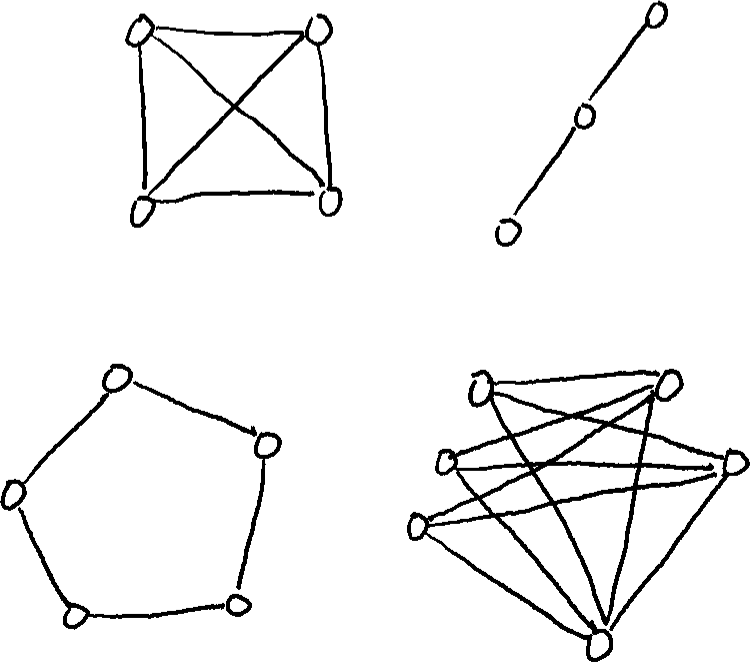
\includegraphics[width=0.5\textwidth]{graphics/L3_trees/graph_families.png}
  \caption[][0cm]{Four graphs: $K_4$, $P_2$, $C_5$, and $K_{3,2,1}$.}
  \label{fig:graph_families}
\end{figure}

\begin{enumerate}
  \item The complete graphs on $n$ vertices, denoted $K_n$. These contain all the $\binom{n}{2}$ potential edges. These are also called \emph{cliques} when we see them as subgraphs of a bigger graph.
  \item The paths of length $\ell$, denoted $P_\ell$. If we take the set $\{0,1,\ldots,\ell\}$ to be our vertex set, the edges are precisely of the form $\{i-1,i\}$ for $i \in [\ell]$.\sidenote[][]{This is another notation you might not have seen before: For an integer $n$, we write $[n]$ for the set $\{1, 2, \ldots, n\}$}
  \item The cycle graphs on $n$ vertices, denoted $C_n$. We can think of these as a path of length $n-1$ with an extra edge joining the first and last vertex.
  \item The complete bipartite graphs on $a + b$ vertices, denoted $K_{a,b}$. These have as vertex set the disjoint union of two sets $L$ and $R$,\sidenote[][]{Think of these as the ``left'' and ``right'' vertices.} with $\abs{L} = a$ and $\abs{R} = b$, and there is an edge between $v$ and $w$ whenever $v \in L$ and $w \in R$. When we see these graphs as subgraphs of a bigger graph, we sometimes also call them \emph{bicliques}.
  \item Generalizing the complete bipartite graphs, the complete multipartite graph on $r$ parts with sizes $a_1, a_2, \ldots a_r$, denoted $K_{a_1, a_2, \ldots, a_r}$, has as its vertex set the disjoint union of $r$ sets $V_1, V_2, \ldots, V_r$, where $\abs{V_i} = a_i$, and there is an edge between two vertices whenever they are not in the same part. We can notice that when $r=2$ this is a complete bipartite graph, and when all the parts are of size $1$ this is a complete graph.
\end{enumerate}

For most of these, it is obvious how many edges they will have. Let us state a lemma that shows how many the complete multipartite graphs have.

\begin{lemma}
  The complete multipartite graph $K_{a_1, a_2, \ldots, a_r}$ has $\frac{1}{2}\left(n^2 - a_1^2 - \ldots - a_r^2\right)$ edges.

  \begin{proof}
    We use the handshake lemma from the previous lecture. Since a vertex in $V_i$ has one edge to every vertex not in $V_i$, it has degree $n - a_i$, and there are $a_i$ such vertices. Thus we can compute that
    \begin{align*}
      2\abs{E} &= \sum_{v\in V} d_v
      = \sum_{i=1}^r \sum_{v \in V_i} d_v\\
      &= \sum_{i=1}^{r} \sum_{v \in V_i} (n - a_i)
      = \sum_{i=1}^{r} a_i(n - a_i)\\
      &= n\left(\sum_{i=1}^{r} a_i\right) - \sum_{i=1}^{r} a_i^2
      = n^2 - \sum_{i=1}^{r} a_i^2
    \end{align*}
    proving the claim.
  \end{proof}
\end{lemma}

\begin{corollary}
  The complete bipartite graph $K_{a,b}$ has $\frac{1}{2}\left(n^2 - a^2 - b^2\right) = ab$ edges.
\end{corollary}

\section{Trees}

\section{Exercises}

%\bibliography{references}
%\bibliographystyle{plainnat}

\end{document}
